% Source: Code/xband-radar-sim/docs/radar_simulation_technical.tex
% Description: Two-ray multipath geometry. The direct path interferes with the ground-reflected path, causing constructive or destructive interference depending on path difference.

\documentclass[border=4pt]{standalone}
\usepackage{algpseudocode}
\usepackage{amsmath,amssymb,amsfonts}
\usepackage[T1]{fontenc}
\usepackage{graphicx}
\usepackage{pgfplots}
\usepackage{tikz}
\usepackage{xcolor}
\pgfplotsset{compat=1.18}
\usetikzlibrary{arrows.meta,positioning,shapes.geometric,calc,patterns,decorations.pathmorphing,3d,angles,quotes}

\definecolor{radargreen}{RGB}{0,255,0}
\definecolor{raycolor}{RGB}{255,165,0}
\definecolor{targetcolor}{RGB}{255,0,0}
\definecolor{groundcolor}{RGB}{139,90,43}
\definecolor{skycolor}{RGB}{135,206,235}
\definecolor{beamcolor}{RGB}{255,255,0}


\begin{document}
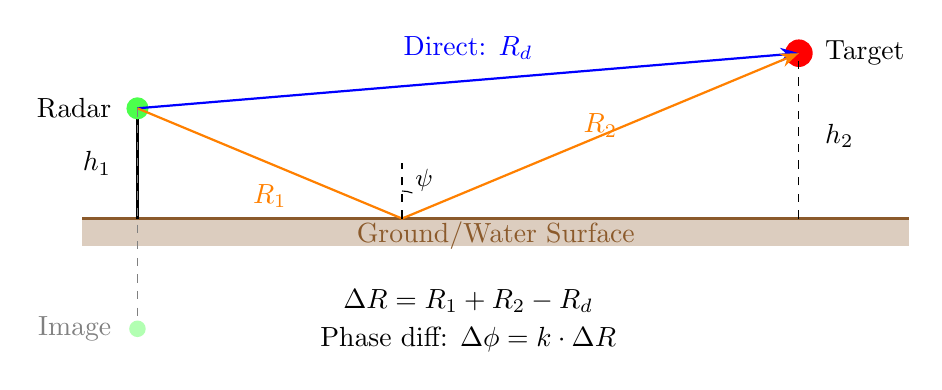
\begin{tikzpicture}[scale=0.7]
    % Ground
    \fill[groundcolor!30] (-1,-0.5) rectangle (14,0);
    \draw[thick, groundcolor] (-1,0) -- (14,0);
    \node[groundcolor] at (6.5,-0.3) {Ground/Water Surface};

    % Radar
    \draw[thick] (0,0) -- (0,2);
    \fill[green!70] (0,2) circle (0.2);
    \node[left] at (-0.3,2) {Radar};
    \node[left] at (-0.3,1) {$h_1$};

    % Target
    \fill[red] (12,3) circle (0.25);
    \node[right] at (12.3,3) {Target};
    \node[right] at (12.3,1.5) {$h_2$};
    \draw[dashed] (12,0) -- (12,3);

    % Direct path
    \draw[thick, blue, -{Stealth}] (0,2) -- (12,3);
    \node[blue, above, sloped] at (6,2.7) {Direct: $R_d$};

    % Reflected path
    \coordinate (reflect) at (4.8,0);
    \draw[thick, orange] (0,2) -- (reflect);
    \draw[thick, orange, -{Stealth}] (reflect) -- (12,3);
    \node[orange, below, sloped] at (2.4,0.8) {$R_1$};
    \node[orange, above, sloped] at (8.4,1.3) {$R_2$};

    % Reflection angle
    \draw[dashed] (reflect) -- ++(0,1);
    \draw ($(reflect)+(0,0.5)$) arc (90:68:0.5);
    \node at ($(reflect)+(0.4,0.7)$) {\small $\psi$};

    % Image
    \draw[dashed, gray] (0,2) -- (0,-2);
    \fill[green!30] (0,-2) circle (0.15);
    \node[gray, left] at (-0.3,-2) {Image};

    % Path difference annotation
    \node at (6,-1.5) {$\Delta R = R_1 + R_2 - R_d$};
    \node at (6,-2.2) {Phase diff: $\Delta\phi = k \cdot \Delta R$};

\end{tikzpicture}
\end{document}
